\documentclass{article}
\usepackage[utf8]{inputenc}
\usepackage{amsmath}
\usepackage{amssymb}
\usepackage{amsthm}
\usepackage{cancel}
\usepackage[shortlabels]{enumitem}
\usepackage{caption}
\usepackage{graphicx}
\usepackage[top=0.6in, bottom=0.6in, left=1in, right=1in]{geometry}
\usepackage{float}

% \usepackage{titlesec}
%     \titlespacing{\subsection}{\parindent}{15pt}{12pt}

\title{\textbf{\underline{CSCI4150U: Data Mining}\\Lab 03}}
\author{Syed Naqvi\\100590852}
\date{\today}

\begin{document}

    \maketitle
    

    \section*{Preprocessing:}

    We start by standardizing the features and visualizing their distributions.

    \begin{figure}[H]
        \centering
        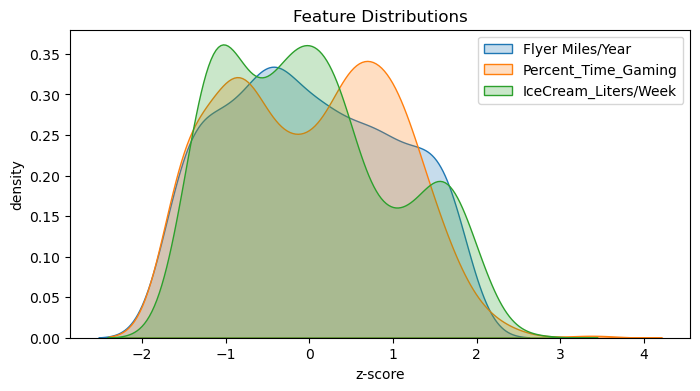
\includegraphics[width=0.5\textwidth, height=0.21\textheight]{pre_a.png}
        \caption{\small{Standardized Distributions}}
    \end{figure}
    \begin{figure}[H]
        \centering
        \begin{minipage}[t]{0.47\textwidth}
            \centering
            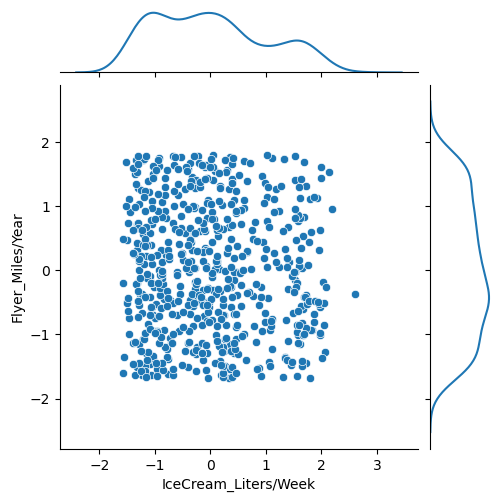
\includegraphics[width=\textwidth, height=0.3\textheight]{pre_c.png}
            \caption{\small{Flyer Miles/Year vs Ice Cream Liters/week}}
        \end{minipage}
        \hfill
        \begin{minipage}[t]{0.47\textwidth}
            \centering
            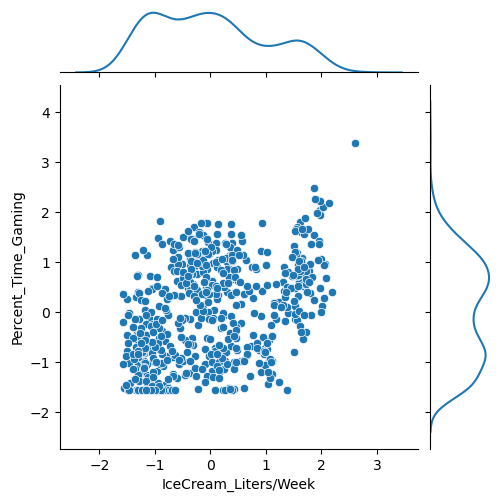
\includegraphics[width=\textwidth, height=0.3\textheight]{pre_b.png}
            \caption{\small{Percentage Time Gaming vs Ice Cream Liters/week}}
        \end{minipage}
    \end{figure}
    \begin{figure}[H]
        \centering
        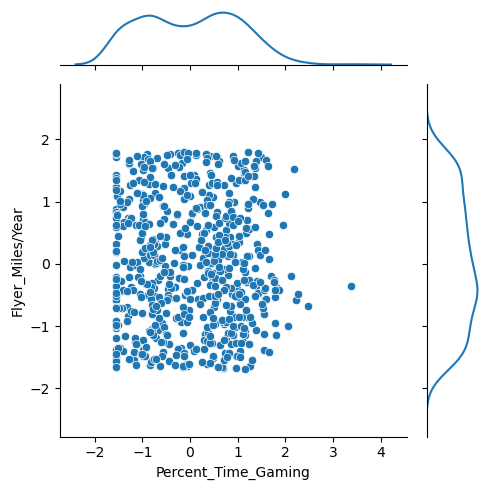
\includegraphics[width=0.6\textwidth, height=0.3\textheight]{pre_d.png}
        \caption{\small{Flyer Miles/Year vs Percentage Time Gaming}}
    \end{figure}

    We can also define a general cross validation helper function and store frequent performance metrics in a dictionary:

    \begin{figure}[H]
        \centering
        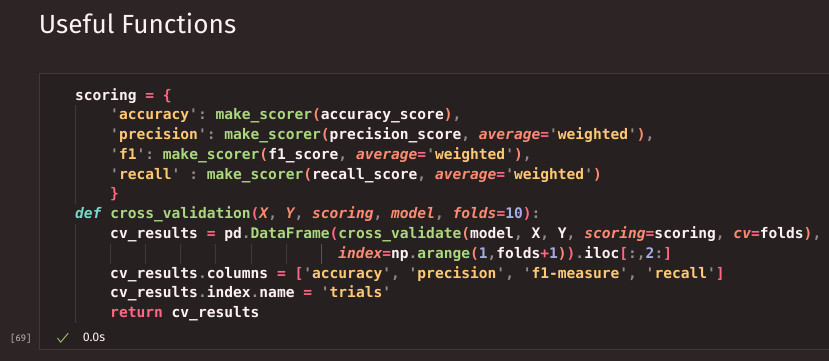
\includegraphics[width=0.7\textwidth, height=0.2\textheight]{helper.png}
        \caption{\small{Utility Functions}}
    \end{figure}

    \newpage

\section*{Naive Bayes Classification (Gaussian Distribution)}

    \subsection*{Validation}

    Although some correlation can be observed between \textbf{Percentage Time Gaming} and \textbf{Ice Cream Liters/week},
    Gaussian Naive Bayes remains a robust classification method due to the roughly normal feature distributions
    and week/nonexistent overall feature pair correlations.

    \begin{figure}[H]
        \centering
        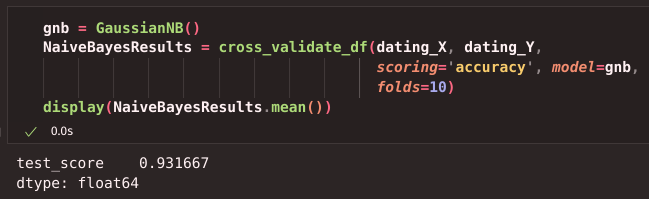
\includegraphics[width=0.7\textwidth, height=0.2\textheight]{NB_results.png}
        \caption{\small{Naive Bayes Cross Validation Results}}
    \end{figure}

\section*{K-NN Classification}

    \subsection*{Model Selection}

    We evaluate test accuracy for k-NN models using different values of \textbf{k}, shuffling the dataset for each
    \textbf{k} value and repeating this process over 100 epochs to determine the best hyperparameter value. Our
    tests help us determine the best value for k should be 5.
    
    \begin{figure}[H]
        \centering
        \begin{minipage}[t]{0.45\textwidth}
            \centering
            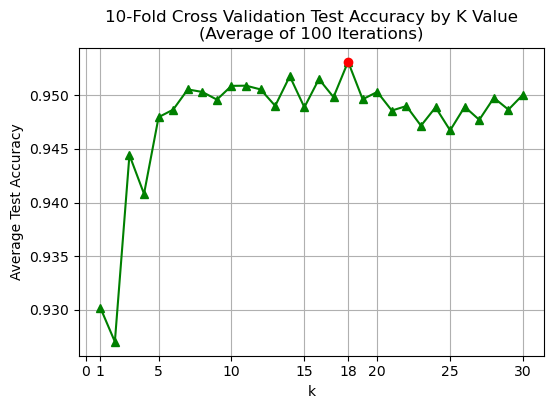
\includegraphics[width=\textwidth, height=0.2\textheight]{k-NN_selection.png}
            \caption{\small{Best K Hyperparameter Selection Barplot}}
        \end{minipage}
        \hfill
        \begin{minipage}[t]{0.54\textwidth}
            \centering
            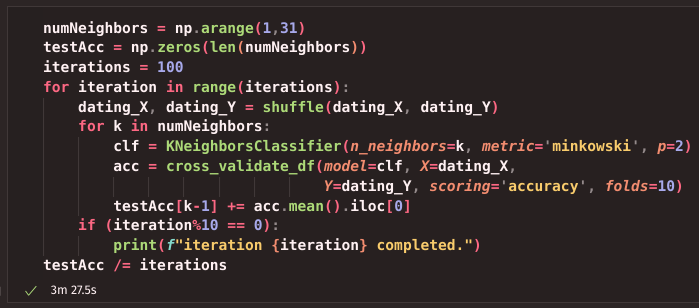
\includegraphics[width=\textwidth, height=0.25\textheight]{k-NN_selection_code.png}
            \caption{\small{Best K Hyperparameter Selection Code}}
        \end{minipage}
    \end{figure}

    \newpage

    \subsection*{Validation}

    Having selecting our model, we perform a 10-fold cross validation and determine the associated average performance
    metrics.

    \begin{figure}[H]
        \centering
        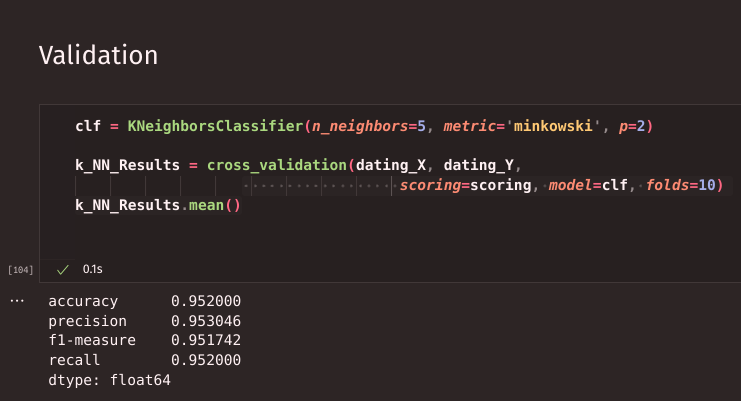
\includegraphics[width=0.7\textwidth, height=0.2\textheight]{k-NN_validation.png}
        \caption{\small{k-NN Cross Validation Results (k=5)}}
    \end{figure}


    \newpage

    \subsection*{2.}

\end{document}